% !TEX TS-program = pdflatex
% !TEX root = RicOp2.tex

\documentclass[a4paper,twoside,openright,titlepage,
               headinclude,,footinclude,BCOR5mm,
               numbers=noenddot,cleardoublepage=empty,
               tablecaptionabove]{scrreprt}
               
\usepackage[T1]{fontenc}
\usepackage[utf8]{inputenc}
\usepackage[english]{babel}
\usepackage{amsmath,amssymb}
\usepackage{indentfirst}
\usepackage[style=philosophy-modern,hyperref]{biblatex}
%\usepackage{biblatex}
\addbibresource{Bibliography.bib}
\usepackage[toc,page]{appendix}
\usepackage{chngpage}
\usepackage{multirow}
\usepackage{calc}
\usepackage{listings}
\usepackage{graphicx}
\usepackage{subfig}
\usepackage{lipsum}
\usepackage{shapepar}
\usepackage{pifont}
\usepackage[eulerchapternumbers,subfig,beramono,eulermath,pdfspacing,listings]{classicthesis}
\usepackage{arsclassica}
\usepackage{tabto}
\usepackage{amsmath}
\usepackage{algorithm}
\usepackage{algorithmic}
\usepackage{booktabs}
%\usepackage{minitoc}
\newenvironment{changemargin}[2]{%
\begin{list}{}{%
\setlength{\topsep}{0pt}%
\setlength{\oddsidemargin}{#1}%
\setlength{\hoffset}{#2}%\\
\setlength{\listparindent}{\parindent}%
\setlength{\itemindent}{\parindent}%
\setlength{\parsep}{\parskip}%
}%
\item[]}{\end{list}}

% ********************************************************************
% Personal commands
% ******************************************************************** 
\newcommand{\myName}{Lorenzo Pantieri}
\newcommand{\myTitle}{The ArsClassica package}
\newcommand{\mySubTitle}{Ah homage to the Elements of Typographic Style}

\DeclareRobustCommand*{\clsname}[1]{{\normalfont\sffamily#1}}
\DeclareRobustCommand*{\pkgname}[1]{{\normalfont\sffamily#1}}
\DeclareRobustCommand*{\optname}[1]{{\normalfont\ttfamily#1}}
\DeclareRobustCommand*{\cmdname}[1]{\mbox{\lstinline[basicstyle=\normalsize\ttfamily]!\\#1!}}

\DeclareRobustCommand*{\classicthesis}{Classic\-Thesis}
\DeclareRobustCommand*{\arsclassica}{{\normalfont\sffamily ArsClassica}}


% ********************************************************************
% Hyper-references
% ******************************************************************** 
\newcommand{\mail}[1]{\href{mailto:#1}{\texttt{#1}}}


% ********************************************************************
% Graphics
% ********************************************************************
\graphicspath{{Graphics/}}


% ********************************************************************
% Code
% ********************************************************************
\definecolor{lightergray}{gray}{0.99}

\lstset{language=[LaTeX]Tex,
     keywordstyle=\color{RoyalBlue},
     basicstyle=\small\ttfamily,
     commentstyle=\color{Emerald}\ttfamily,
     stringstyle=\rmfamily,
     numberstyle=\scriptsize,
     showstringspaces=false,
     breaklines=true,
     frame=lines,
     backgroundcolor=\color{lightergray},
     flexiblecolumns=true,
     escapeinside={�*}{*�},
     firstnumber=last,
} 

\newcommand{\meta}[1]{$\langle${\normalfont\itshape#1}$\rangle$}

\lstset{	morekeywords=%
    {ProvidesPackage,RequirePackage,areaset,ifthenelse,%
     chapterNumber,undefined,boolean,DeclareRobustCommand,%
     spacedallcaps,textssc,MakeTextUppercase,lehead,%
     microtypesetup,textls,spacedlowsmallcaps,MakeTextLowercase,%
     sodef,allcapsspacing,lowsmallcapsspacing,thesection,%
     color,headmark,rohead,headfont,pnumfont,titleformat,%
     part,partname,thepart,chapter,thechapter,titlerule,%
     subsection,thesubsection,subsubsection,thesubsubsection,%
     paragraph,theparagraph,descriptionlabel,titlespacing,%
     formatchapter,textcolor,clearscrplain,rofoot,labelitemi,
     captionsetup,hypersetup}}

\lstnewenvironment{code}% 
   {\setkeys{lst}{columns=fullflexible,keepspaces=true}%
   \lstset{basicstyle=\small\ttfamily}}{}


% ********************************************************************
% Bibliography
% ******************************************************************** 
\bibliography{Bibliography}

\defbibheading{bibliography}{%
\cleardoublepage
\manualmark
\phantomsection
\addcontentsline{toc}{chapter}{\tocEntry{\bibname}}
\chapter*{\bibname\markboth{\spacedlowsmallcaps{\bibname}}
{\spacedlowsmallcaps{\bibname}}}}

\renewcommand*{\nameyeardelim}{\addcomma\space}

\begin{document}
%\dominitoc
%\dominilof
%\dominilot
%\faketableofcontents
%\fakelistoffigures
%\fakelistoftables
\pagenumbering{roman}
\pagestyle{plain}
% !TEX TS-program = pdflatex
% !TEX root = ../ArsClassica.tex
%*******************************************************
% Titlepage
%*******************************************************
\begin{titlepage}
\pdfbookmark{Titlepage}{Titlepage}
\changetext{}{}{}{((\paperwidth  - \textwidth) / 2) - \oddsidemargin - \hoffset - 1in}{}
    \begin{center}

	\begin{center}
	
\includegraphics[scale=0.08]{Graphics/unipd.png}
	\end{center}
	
	\vspace{0.2in}	
	\textsc{\LARGE Università degli Studi di Padova}\\[1.5cm]
    \vspace{1.3in}
    \Huge \textmd{\textbf{Wind Farm Cable Problem}}\\
	\vspace{0.1in}   
    \Large Advanced combinatorial optimization algorithms \\
    \Large Ricerca Operativa 2\\
    \vspace{1in}
	\NumTabs{6}
	\begin{minipage}{5cm} 
	\centering
	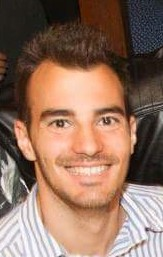
\includegraphics[scale=0.5]{Graphics/Foto.jpg} \\
	\textbf{Piona Davide} \\	
	\textbf{1149616}
	\end{minipage}
	\begin{minipage}{5cm} 
	\centering
	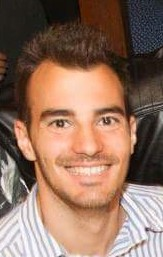
\includegraphics[scale=0.5]{Graphics/Foto.jpg} \\
	\textbf{Benini Michele} \\	
	\textbf{1139089}
	\end{minipage}
 	\vspace{1in}
 	\\	
	\Large Academic Year 2017-2018\\
	
  	                    

    \end{center}        
\end{titlepage} 
%% !TEX TS-program = pdflatex
% !TEX root = ../ArsClassica.tex

%*******************************************************
% Titleback
%*******************************************************
\thispagestyle{empty}
\pdfbookmark{Titleback}{Titleback}

\hfill

\vspace{\stretch{2}}

\begin{center}
Lorenzo Pantieri \\
\smallskip
\textit{The \arsclassica{} package}\\
\smallskip
Copyright\,\textcopyright\ 2008-2017
\end{center}
\vspace{\stretch{1}}

\medskip

\noindent\textsf{\spacedlowsmallcaps{Titleback}} \\
\noindent
This document was written with \LaTeX{} on Mac using \arsclassica, a reworking of the \classicthesis{} style designed by Andr\'e Miede, inspired to the masterpiece \emph{The Elements of Typographic Style} by Robert Bringhurst. 

\bigskip

\noindent
\textsf{\spacedlowsmallcaps{Contacts}}

\noindent
{\raisebox{-0.33ex}{\ding{43}}}\,\mail{lorenzo.pantieri@gmail.com}
\cleardoublepage
\pagestyle{scrheadings} 
% !TEX TS-program = pdflatex
% !TEX root = ../ArsClassica.tex

%*******************************************************
% Contents
%*******************************************************
\phantomsection
\pdfbookmark{\contentsname}{tableofcontents}
\setcounter{tocdepth}{2}
\tableofcontents
\markboth{\spacedlowsmallcaps{\contentsname}}{\spacedlowsmallcaps{\contentsname}} 
\cleardoublepage
\pagenumbering{arabic}
%% !TEX TS-program = pdflatex
% !TEX root = ../ArsClassica.tex

%************************************************
\chapter{Fundamentals}
\label{chp:fundamentals}
%************************************************

This chapter introduces the (truly simple) basic notions of \arsclassica{} and presents its fundamental ideas and distinctive features.



\section{Introduction}

The \arsclassica{} package changes some features of the \classicthesis{} style, designed by Andr\'e Miede. It allows to reproduce the layout of the \LaTeX{} guide \emph{The Art of Writing with \LaTeX}~\parencite{pantieri:arte} and of this document.

\section{Use}

This package is shaped to be executed on a \emph{complete} installation of \TeX{}~Live or MiK\TeX, and uses freely available fonts.
It works with the \clsname{KOMA-Script} classes (\clsname{scrreprt}, \clsname{scrbook} and \clsname{scrartcl}) and requires the \pkgname{classicthesis} package. \arsclassica{} must be loaded \emph{after} \pkgname{classicthesis}:
\begin{code}
\documentclass[�*\meta{\dots\unkern}*�]{scrreprt} % or scrbook or scrartcl

\usepackage[�*\meta{\dots\unkern}*�]{classicthesis}
\usepackage{arsclassica}

\begin{document}
�*\dots*�
\end{document}
\end{code}

For example, this document has been produced with the following code:
\begin{code}
\documentclass[a4paper,twoside,openright,titlepage,
               headinclude,footinclude,BCOR5mm,
               numbers=noenddot,cleardoublepage=empty,
               tablecaptionabove]{scrreprt}

\usepackage{�*\meta{\dots\unkern}*�}
\usepackage{subfig}
\usepackage[eulerchapternumbers,subfig,beramono,eulermath,pdfspacing]%
           {classicthesis}
\usepackage{arsclassica}

\begin{document}
�*\dots*�
\end{document}
\end{code}

It is recommended to use the \optname{beramono} and \optname{eulerchapternumbers} options together with \arsclassica.



\section{Style}

The typographical style achieved with \arsclassica{} differs from \classicthesis{} in the following points:
\begin{itemize}
\item use of Iwona font, by Janusz Nowacki, for the sectioning unit titles (chapters, sections, subsections, sub-subsections, paragraphs and subparagraphs), for the description list labels, the headlines and the caption labels (\classicthesis{} doesn't use any sans serif font);
\item customized chapter numbers;
\item semi-transparent headlines; the headlines are separated from the page number by a small rule;
\item caption labels in boldface (\classicthesis{} doesn't use any boldface font);
\item itemize lists with semi-transparent bullets.
\end{itemize}

\arsclassica{} is designed  to provide a ready-to-use typographical style: for this reason it has no loading options and it is \emph{not} configurable or customizable in any way. If you change the previous settings, you'll risk to destroy the balance of the style, so it is \emph{highly recommended} to keep them unchanged.

One of the principles of \LaTeX{} is that it allows the author to take no interest in the typographical questions, permitting him to focus only on the structure and the contents of his document. This fact should always be kept in mind: using a style written by others, the user accepts all the typographical settings chosen for him by the author of the style, and he isn't forced to study typography to fine-tune the layout of his publications. This is the case of \arsclassica{} too: if you change its settings, you'll deny this philosophy and, consequently, you'll have to study (a lot of) typography to achieve acceptable results. 

The style achieved with \arsclassica{} is \emph{not} therefore configurable or customizable. The typographical style is very personal: if you like this package and find attractive the idea to take no interest in the problem of the style definition, then you'll use \arsclassica{} with satisfaction; otherwise, if you have different needs or you aren't satisfied with the layout of the package, then you should try other classes or packages, even building your own style.



\section{Important}

To write a document according to the \arsclassica{} style, you have to follow some very simple rules.
\begin{itemize}
\item Don't change \emph{for any reason} the \arsclassica{} settings (fonts, text body size, colors, \dots).
\item The sectioning unit titles (chapters, section, subsections, \dots) have to be \emph{one line long}, possibly in \emph{plain text} (no symbols, formulas or code fragments). If you have titles longer than one line, try and rephrase them: you can almost always do it.
\item In the table of contents and in the list of tables and figures, captions have to be \emph{one line long}, possibly in \emph{plain text}. Use the optional argument of sectioning commands and of \cmdname{caption}, if necessary.
\item Don't use \optname{tocaligned} and \optname{dottedtoc} options of \classicthesis: the default table of contents does the job very well (see the documentation of \classicthesis{} for a nice discussion of this point).
\item Don't use vertical or double rules in your tables (see the documentation of \pkgname{booktabs}).
\item Use footnotes and margin notes very sparingly.
\item If your document includes graphs and plots, draw them using \LaTeX{} (by \pkgname{Ti\emph{k}Z} and \pkgname{pgfplots}, for example) and not an external software. This is the only way to get the best typographical outcome. 
\end{itemize}


 
\section{Examples}

\begin{figure}
\centering
\subfloat[Asia personas duo]
{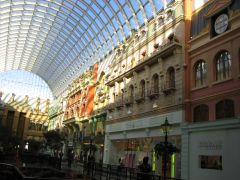
\includegraphics[width=.45\columnwidth]{Lorem}} \quad
\subfloat[Pan ma signo]
{\label{fig:example-b}%
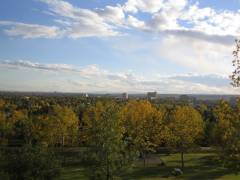
\includegraphics[width=.45\columnwidth]{Ipsum}} \\
\subfloat[Methodicamente o uno]
{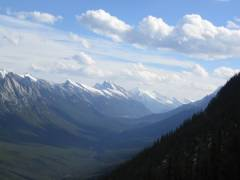
\includegraphics[width=.45\columnwidth]{Dolor}} \quad
\subfloat[Titulo debitas]
{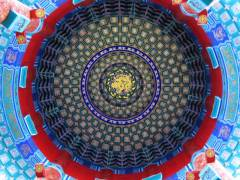
\includegraphics[width=.45\columnwidth]{Sit}}
\caption[Tu duo titulo debitas latente]{Tu duo titulo debitas latente}
\label{fig:example}
\end{figure}

Please note that the content of this section is just some dummy text. It isn't a real language.

Lorem ipsum dolor sit amet, consectetuer adipiscing elit. Ut purus elit, vestibulum ut, placerat ac, adipiscing vitae, felis. Curabitur dictum gravida mauris.

\subsection*{A subsection}

\lipsum[2]

\subsubsection*{A sub-subsection}

\lipsum[7]

\paragraph{A paragraph}
Lorem ipsum dolor sit amet, consectetuer adipiscing elit. Ut purus elit, vestibulum ut, placerat ac, adipiscing vitae, felis. Curabitur dictum gravida mauris. Nam arcu libero, nonummy eget, consectetuer id, vulputate a, magna.

\paragraph{Another paragraph}
Cras nec ante, pellentesque a nulla, cum sociis natoque penatibus et magnis dis parturient montes, nascetur ridiculus mus. Aliquam tincidunt urna

\bigskip

Donec aliquet, tortor sed accumsan bibendum, erat ligula aliquet magna, vitae ornare odio metus a mi. Morbi ac orci et nisl hendrerit mollis. Suspendisse ut massa. Cras nec ante. Pellentesque a nulla. Cum sociis natoque penatibus et magnis dis parturient montes, nascetur ridiculus mus. Aliquam tincidunt urna.

\begin{description}
\item[Mane] Lorem ipsum dolor sit amet, consectetuer adipiscing elit. 
\item[Tekel] Ut purus elit, vestibulum ut, placerat ac, adipiscing vitae, felis. Curabitur dictum gravida mauris.
\item[Fares] Nam arcu libero, nonummy eget, consectetuer 
id, vulputate a, magna.
\end{description}

\begin{table}
\caption{Lorem ipsum dolor sit amet}
\centering
\begin{tabular}{ll}
\toprule
\textbf{Alkaloid} & \textbf{Origin} \\
\midrule
atropine & belladonna \\
morphine & poppy \\
nicotine & tobacco \\
\bottomrule
\end{tabular}
\end{table}

Suspendisse vel felis. Ut lorem lorem, interdum eu, tincidunt sit amet, laoreet vitae, arcu. Aenean faucibus pede eu ante. Praesent enim elit, rutrum at, molestie non, nonummy vel, nisl. Ut lectus eros, malesuada sit amet, fermentum eu, sodales cursus, magna. Donec eu purus. Quisque vehicula, urna sed ultricies auctor, pede lorem egestas dui, et convallis elit erat sed nulla.

\subsection*{Some formulas}

Una formula in linea viene incorporata nel testo: $\lim_{n \to \infty}\sum_{k=1}^n \frac{1}{k^2} = \frac{\pi^2}{6}$, per esempio. Come si osserva, \LaTeX{} fa \emph{il possibile} per comprimerla e modificare il meno possibile l'interlinea nel capoverso che la contiene.
Una formula in display viene invece composta da \LaTeX{} su linee a parte, separate dal contesto con adeguati spazi bianchi per metterla in mostra e farla risaltare sulla pagina.
\begin{equation}
\lim_{n \to \infty}\sum_{k=1}^n \frac{1}{k^2}= \frac{\pi^2}{6}
\end{equation}
Come si osserva, ora la formula risulta centrata, non compressa, e tutti i suoi elementi occupano il giusto spazio con un risultato finale di grande respiro.

Integer tempus convallis augue. Etiam facilisis. Nunc elementum fermentum wisi. Aenean placerat. Ut imperdiet, enim sed gravida sollicitudin, felis odio placerat quam, ac pulvinar elit purus eget enim. 

\begin{equation}
\int_a^{a+T}f(x)\,dx= \int_0^T f(x)\,dx 
\qquad
\oint f(z)\,dz=2\pi i
\end{equation}

Nulla malesuada porttitor diam. Donec felis erat, congue non, volutpat at, tincidunt tristique, libero. Vivamus viverra fermentum felis. Donec non- ummy pellentesque ante.

\begin{equation}
f(x_1,\dots,x_n)=  \prod_{k=1}^n x_k 
\qquad
\sum_{k=1}^n x_k^2=1
\qquad
\biggl(\sum_n x_n^2\biggr)^{1/2} 
\end{equation}

\lipsum[2]

\begin{equation}
\begin{bmatrix} 
a_{11} & \dots & a_{1n} \\ 
a_{21} & \dots & a_{2n} \\ 
\hdotsfor{3} \\ 
a_{n1} & \dots & a_{nn} 
\end{bmatrix}
\end{equation}

\lipsum[4]

\begin{equation}
\lim_{x\to 0}
\frac{\sin x}{x}=1 \qquad
\lim_{n\to +\infty}f_n=\delta
\end{equation}

Fusce mauris. Vestibulum luctus nibh at lectus. Sed bibendum, nulla a faucibus semper, leo velit ultricies tellus, ac venenatis arcu wisi vel nisl. Vestibulum diam.

\begin{equation}
n!=
\begin{cases} 
1       & \text{if $n=0$} \\ 
n(n-1)! & \text{if $n\ge 1$} 
\end{cases} 
\end{equation}

Ut lectus eros, malesuada sit amet, fermentum eu, sodales cursus, magna. Donec eu purus. Quisque vehicula, urna sed ultricies auctor, pede lorem egestas dui, et convallis elit erat sed nulla. Donec luctus. Curabitur et nunc. Aliquam dolor odio, commodo pretium, ultricies non, pharetra in, velit.

\begin{equation} 
x_G=
\frac{\displaystyle
      \sum_{i=1}^n m_ix_i}
{\displaystyle\sum_{i=1}^n m_i}
\end{equation}

\lipsum[6]

\begin{equation}
\kappa =\frac{\xi}{E_{\textrm{max}}}
\qquad
E_{\textup{max}} =\frac{2 m_{\textup{e}} \beta^2\gamma^2 }{1 +2\gamma m_{\textup{e}}/m_{\textrm{x}} + ( m_{\textup{e}}/m_{\textup{x}})^2}
\end{equation}

\lipsum[8]
% !TEX TS-program = pdflatex
% !TEX root = ../ArsClassica.tex

%************************************************
\chapter{Development Environment}
\label{chp:1-Environment}
%************************************************
To allow replicability of our experiments, we have added some information about the system and the environment that we used for our research. 
We used the following development environment:
\begin{itemize}
\item \textsc{CPLEX} :  version 0.1-2018
\item \textsc{Linux Ubuntu} : version 18.04 LTS (Operative System)
\item \textsc{C}  	(language)
\item \textsc{Sublime text} (IDE / text editor)
\item \textsc{Github} (web-based version control using Git)
\item \textsc{Gnuplot} (library plot)
\end{itemize}

\section{Real World Info}
As in [\cite{wfcp}] research, we used a library of real-life instances that are publicly available for benchmarking.
For benchmark purposes, we collected the data of five real wind farms in operation in United Kingdom (wf02, wf03, wf05) and Denmark (wf01, wf04). Different types of cable with different costs, capacities and electrical resistances are available on the market; we considered 5 sets of real cables, named cb01, cb02, cb03, cb04, and cb05. The turbines in each wind park are of the same type, so we can express the cable capacities as the maximum number of turbines that it can support. Finally, we list the maximum number of connections to the substation, or to be specific, the input parameter C. The table 1 contains all the information.
\begin{table}[!htbp]\label{tab:realWorld}
\center
\begin{tabular}{llllll}
\hline
name & site         & turbine type  & no. of turbines & C  & allowed cables      \\ \hline
wf01 & Horn Rev 1   & Vestas 80-2MW & 80              & 10 & cb01-cb02-cb05      \\
wf02 & Kentis Flats & Vestas 90-3MW & 30              & $\infty$   & cb01-cb02-cb04-cb05 \\
wf03 & Ormonde      & Senvion 5MW   & 30              & 4  & cb03-cb04           \\
wf04 & DanTysk      & Simens 3.6MV  & 80              & 10 & cb01                \\
wf05 & Thanet       & Vestas 90-3MW & 100             & 10 & cb04-cb05           \\ \hline
\end{tabular}
\caption{Basic information on the real-world wind farms that were used for testing.}
\end{table}

\section{Instance TEST BED}
The test that we were able to use are the combinations between the 5 instances of wind farms and the 5 sets of real cables. For simplicity reasons and in order to eliminate mistakes, we adopted the same a numeration as the [\cite{wfcp}] article. This solution allows us to easily compare our results with the results in that research. 
Table 2 reports the resulting numbers of the different instances. For example we renamed the 01 wind farm as \textit{data\_01.turb} and the corresponding cables as \textit{data\_01.cbl}. Figures \ref{img:ex1} and \ref{img:ex2} shows two instances from TEST BED.

\begin{table}[!htbp]\label{tab:testBed}
\center
\begin{tabular}{lcl}
\hline
number & \multicolumn{1}{l}{wind farm} & cable set         \\ \hline
01     & \multirow{6}{*}{wf01}         & wf01\_cb01\_capex \\
02     &                               & wf01\_cb01        \\
03     &                               & wf01\_cb02\_capex \\
04     &                               & wf01\_cb02        \\
05     &                               & wf01\_cb05\_capex \\
06     &                               & wf01\_cb05        \\ \hline
07     & \multirow{8}{*}{wf02}         & wf02\_cb01\_capex \\
08     &                               & wf02\_cb01        \\
09     &                               & wf02\_cb02\_capex \\
10     &                               & wf02\_cb02        \\
12     &                               & wf02\_cb04\_capex \\
13     &                               & wf02\_cb04        \\
14     &                               & wf02\_cb05\_capex \\
15     &                               & wf02\_cb05        \\ \hline
16     & \multirow{4}{*}{wf03}         & wf03\_cb03\_capex \\
17     &                               & wf03\_cb03        \\
18     &                               & wf03\_cb04\_capex \\
19     &                               & wf03\_cb04        \\ \hline
20     & \multirow{2}{*}{wf04}         & wf04\_cb01\_capex \\
21     &                               & wf04\_cb01        \\ \hline
26     & \multirow{4}{*}{wf05}         & wf05\_cb04\_capex \\
27     &                               & wf05\_cb04        \\
28     &                               & wf05\_cb05\_capex \\
29     &                               & wf05\_cb05        \\ \hline
\end{tabular}
\caption {Test Bed instance numbers.}
\end{table}

\begin{minipage}{7cm} 
	\centering
	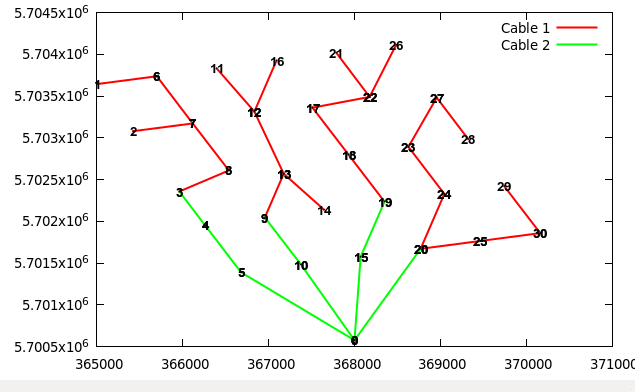
\includegraphics[scale=0.3]{Graphics/data07.png} \\
	\captionof{figure}{Example of problem: data07}
	\label{img:ex1}
	\end{minipage}
	\begin{minipage}{7cm} 
	\centering
	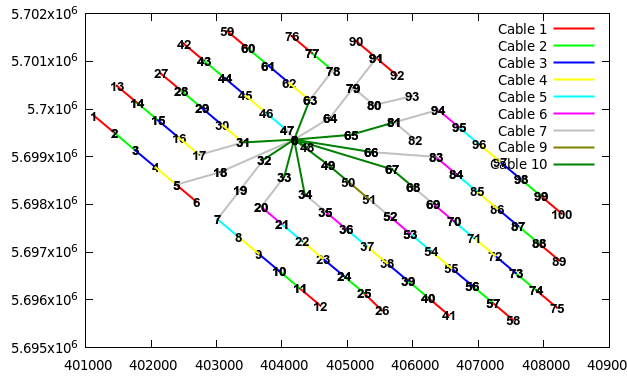
\includegraphics[scale=0.3]{Graphics/data29.png} \\
	\captionof{figure}{Example of problem: data29}
	\label{img:ex2}
	\end{minipage}

\newpage
% !TEX TS-program = pdflatex
% !TEX root = ../ArsClassica.tex

%************************************************
\chapter{Mathematical Model}
\label{chp:2-Model}
%************************************************

\section{Wind Farm Cable Problem Introduction}
We have studied the Wind Farms Cable Problem, which is represented by a number of wind farms in the sea that produces energy; the power production needs to be routed by some cables to the substation and then directed to the coast.
To do that, each turbine must be connected through a cable to another turbine, and eventually to a substation.\\

The problem complexity of the cable routing problem is strongly NP-hard according to \cite{wfcp}. They have proved that the problem is NP-hard in two formulations. First, in the case where all turbines have the same power production and the nodes are not associated with points in the plane. Second, in the case where the turbines can have different power production and are associated with point in the plane. 

When designing a feasible cable routing, it's necessary to take in account a number of constraints. Here we list some of them and then we'll describe the mathematical model that realizes those constraints. Our model is based on the following requirements:

\begin{itemize}
\item since the energy flow is unsplittable, the energy flow leaving a turbine must be supported by a single cable.
\item power losses should be avoided because it will cause revenue losses in the future.
\item different cables, with different capacities and costs are available. This means that it is important to choose the right cable to minimize the costs without affecting the revenues. 
\item the energy flow on each connection cannot exceed the capacity of the installed cable.
\item due to the substation physical layout, a given maximum number of cables, say $C$, can be connected to each substation.
\item cable crossing should be avoided. (we will discuss this problem in the next subsection)
\end{itemize}
Let $K$ denote the number of different types of cables that can be used and let $n$ be the number turbines. 

Definition of $y_{ij}$ :
\[
	y_{ij} =
   \begin{cases}
   1 \quad \mbox{if arc } (i,j) \mbox{ is constructed} \\
   0 \quad \mbox{otherwise.} 
   \end{cases}
   \forall \,i,j = 1, ..., n 
\]
\[
	y_{ii} = 0, \quad \forall i= 1, ... n 
\]
Definition of $x^k_{ij}$ :
\[
	x^k_{ij} =
   \begin{cases}
   1 \quad \mbox{if arc } (i,j) \mbox{ is constructed with cable type k} \\
   0 \quad \mbox{otherwise.} 
   \end{cases}
   \forall \,i,j = 1, ..., n \ \forall \ k = 1,... K
\]
Definition of $f_{ij}$ :
\[
	f_{ij} \geq 0, \quad \forall i,j= 1, ... n
\]

%\[
%y_{i,j} = \sum_{t \in T} x^t_{ij}, \quad (i,j) \in A
%\]
Objective function: 
\begin{equation}\label{eq:obj}
	\min{\sum^n_{i=1} \sum^n_{j=1} \sum^K_{k} cost(k) \cdot dist(i,j) \cdot x^k_{ij}}
\end{equation}

Constraints: 
\begin{equation}\label{eq:numberCable}
	\sum^n_{j = 1} y_{hj} = 
	\begin{cases}
   1 \quad \mbox{if } P_h \geq 0, \quad \forall h=1,...,n \\
   0 \quad \mbox{if } P_h = -1
   \end{cases}
\end{equation}

\begin{equation}\label{eq:basestation}
	\sum^n_{i =1} y_{ih} \leq C, \quad \forall h \ | \ P_h = -1
\end{equation}

\begin{equation}\label{eq:flux}
	\sum^n_{j=1} f_{hj} = \sum^n_{i=1} f_{ih}+ P_h, \quad \forall h \ | \ P_h \geq 0
\end{equation}

\begin{equation}\label{eq:oneCable}
	y_{ij} = \sum^K_{k=1} x^k_{ij}, \quad i,j = 1,...,n
\end{equation}

\begin{equation}\label{eq:capacity}
	\sum^K_{k=1} cap(k)x^k_{ij} \geq f_{ij}, \quad \forall i,j = 1,...,n
\end{equation}

The objective function \ref{eq:obj} minimizes the total cable layout cost, where $dist(i, j)$ is the Euclidean distance between nodes $i$ and $j$ and $cost(k)$ is the unit cost for the cable $k$. 
Constraints \ref{eq:oneCable} impose that only one type of cable can be selected for each build arc.
Constraints \ref{eq:flux} are flow conservation constraints: the energy exiting each node $h$ is equal to the energy entering $h$ plus the power production of the node. 
Constraints \ref{eq:capacity} ensure that the flow does not exceed the capacity of the installed cable.
Constraints \ref{eq:numberCable} impose that only one cable can exit a turbine and that no one cable can exit from the substation. 
Constraint \ref{eq:basestation} imposes the maximum number of cables ($C$) that can enter in a substation, depending on the data of the instance. The image \ref{img:wfcp} shows an example of a graphical solution to the cable routing problem.

\begin{center}
	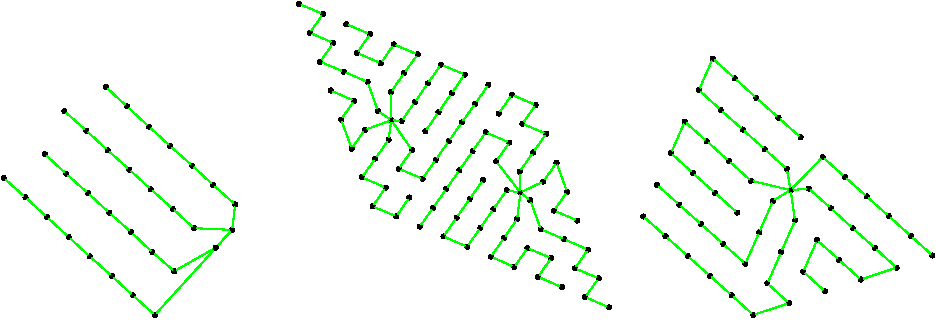
\includegraphics[scale=0.4]{Graphics/wfcp.png}
	\captionof{figure}{Example solutions to a cable routing problem}
	\label{img:wfcp}
\end{center}
	
\section{Crossing Cables}
According to \cite{wfcp}, an important constraint is that cable crossings should be avoided. In principle, cable crossing is not impossible, but is strongly discouraged, in practice as building one cable on top of another is more expensive and increases the risks of cable damages.\\

In order to evaluate if two arches cross, we used the Cramer Method: given the arc $a$ between $P_1$ and $P_2$ and the arc $b$ between $P_3$ and $P_4$. We define the coordinates of a general point as: $P_j = (X_i, y_i)$. \\
Using the Cramer method we have:
\[
{x \choose y} = {x_1 \choose y_1}+ \lambda {x_2 - x_1 \choose y_2 - y_1} \quad \lambda \in \ ]0, 1[
\]   
\[
{x \choose y} = {x_3 \choose y_3}+ \mu {x_4 - x_3 \choose y_4 - y_3} \quad \mu \in \ ]0, 1[
\]    
Then we evaluate if the determinant is equal to zero value. By using a calculator we will check if the determinant is smaller than a constant epsilon with value $\simeq 10^{-9}$. We can have two situations:
\begin{enumerate}
\item if $det=0 \quad \Rightarrow$ no crossing 
\item if $det \neq 0 \quad \Rightarrow (\lambda, \mu) \ if \ (\lambda \in \ ]0, 1[) \ \&\& \ (\mu \in \ ]0, 1[) \Rightarrow $ crossing
\end{enumerate}                                                   

\[
y(a,b)+ y(c,d) \leq 1, \quad \forall (a,b,c,d): [P_a, P_b] \ cross \ [P_c, P_d]
\]


% !TEX TS-program = pdflatex
% !TEX root = ../ArsClassica.tex

%************************************************
\chapter{CPLEX}

\label{chp:3-CPLEX}

%************************************************
\section{Plain Execution}
We simply create the linear programming model and then we pass it to \textsc{CPLEX} for the optimization. The performances, as we will notice for all the methods, depend on the instance. We noticed the power of \textsc{CPLEX} which finds the optimal solution in few seconds, and in the meantime we discovered that some instances take many hours to be solved by our machines. 
The main steps of our code in this phase are: 
\begin{itemize}
\item Read the input files and the command line parameter and parse them;
\item Memorize turbines and cables;
\item Develop the specific linear programming model;
\item Call CPX\_INT\_OPT that optimizes the instance;
\item Ask to \textsc{CPLEX} the optimal function;
\item Print and graph it;
\end{itemize}

\subsection{Relaxed Mode}
Sometimes there are constraints that risk to block the improvement of the solution or make \textsc{CPLEX} take longer before finding a feasible solution. \\
To avoid those situations, it is possible to \textit{"relax"} some constraints in order to speed up the process of searching for the first solution. The main steps are to add a slack variable $\geq 0$ in the model and then add this variable in the objective function multiplied for a constant reasonably large. In this way, even if \textsc{CPLEX} could find a wrong initial solution, it is probable that this solution will rapidly improve and be corrected. Anyway, the choice to relax some constraint should not affect the optimal solution because of the very high impact on the objective function. \\
In our case we found three constraints that could be relaxed: the maximum number $C$ of edges entering in a substation, the flux losses and the need to have one big connected component that connects all the arcs (for some heuristic algorithm). \\
The first constraint can be relaxed in this way (see the result in image \ref{img:relax1}):
\[
f^{R_1}_{obj} (x,y,k) = f_{obj} (x,y,k) + BIG\_M\_CABLE \cdot s
\]
\[
c \geq \sum^n_{i=1} y_{ih} -s \quad \forall \ h : P_h = -1
\]
The second constraint, about the flux losses, can be relaxed in this way (see the result in image \ref{img:relax2}):
\[
f^{R_2}_{obj} (x,y,k) = f_{obj} (x,y,k) + BIG\_M\_CABLE \cdot \sum^n_{i=1} s_i
\]
\[
\sum^n_{i=1} f_{hs} = \sum^n_{i=1} f_{ih} + P_h - s_h \quad \forall h = 1, ... n
\]
And finally it is possible to add to the relaxed constraint $f^{R_2}_{obj} (x,y,k)$ also the third option, simply adding the following constraint (see the result in image \ref{img:relax3}): 
\[
\sum^n_{j=1} y_{ij} < 1 \quad \forall i = 1, ... n
\]
We listed the three different possibility that we can activate in our algorithms. The second and the third options come out of thinking about heuristic algorithm, while the first option can be applied in all the algorithms. 
\begin{center}
	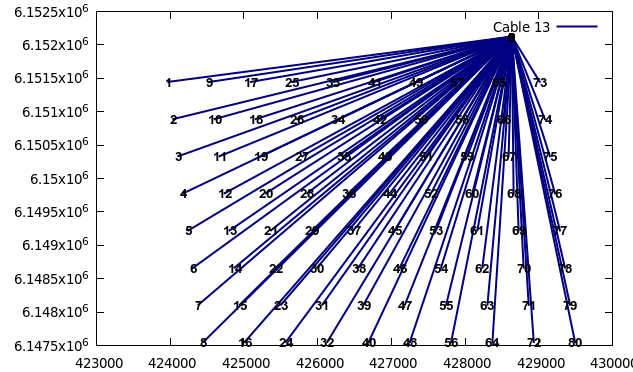
\includegraphics[scale=0.4]{Graphics/data02-relax1.png}
	\captionof{figure}{Example relax 1}
	\label{img:relax1}
\end{center}

\begin{center}
	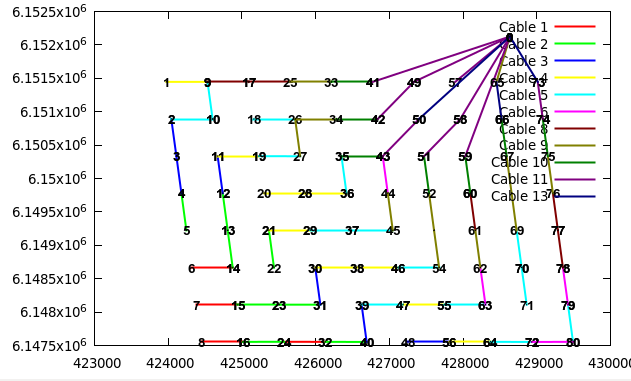
\includegraphics[scale=0.4]{Graphics/data02-relax2.png}
	\captionof{figure}{Example relax 2}
	\label{img:relax2}
\end{center}

\begin{center}
	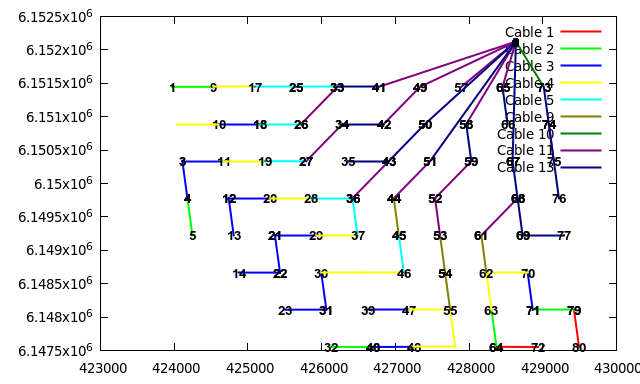
\includegraphics[scale=0.4]{Graphics/data02-relax3.png}
	\captionof{figure}{Example relax 3}
	\label{img:relax3}
\end{center}
\subsection{CPLEX Heuristics-Params}
The \textsc{CPLEX} code contains some heuristic procedures. Being integrated into branch \& cut, they can speed the final proof of optimality or provide a suboptimal but high-quality solution in a shorter amount of time than by branching alone. With default parameter settings, \textsc{CPLEX} automatically invokes the heuristics when they seem likely to be beneficial. However, it is possible to adapt them to our specific case and instances by changing the frequency of activation of these procedures by setting some \textsc{CPLEX} parameter. We mainly analyzed two of them:
\begin{itemize}
\setlength{\parskip}{0pt}
\setlength{\itemsep}{0pt plus 1pt}
\item \textbf{RINS}: it means \textit{Relaxation induced neighborhood search} and it is a heuristic that explores a neighborhood of the current incumbent solution to try to find a new, improved incumbent. In the initial part the process does not change, but as soon as a solution is found the RINS heuristic tries to improve it with more frequency. It is possible to infer that the RINS method has been used in a \textsc{CPLEX} step when in the logs there is a ‘*’ near to the number. We set the \textit{-rins} param to 5 in all the tests. 
\item \textbf{POLISHING}: this heuristic tries to modify some variables of a (good) solution to improve it. It is possible to set a condition that enables this method, in order to avoid premature usage of this method, which that can lead to wasted time and performances. We decided not to change this parameter in our tests.
\end{itemize}

\section{Lazy Constraints Method}
The generated constraints are often too much and risk to block the solution for a long time if we added to the model statically.  
Instead of adding systematically all the constraints in the model at the beginning, we generate them "on the fly" when they are violated by the Branch and Bound process. In this way \textsc{CPLEX} will check those constraints only when a solution is created. In the case that some constraint is violated, \textsc{CPLEX} will add the corresponding constraint before the incumbent update. \\
The \textsc{CPLEX} command to add a set of constraints is \textit{CPXAddLazyConstraints}. \\
This technique decreases the efficiency of the \textsc{CPLEX} pre-processing and sometimes the computation time of the solution is really high, but generally gives good results.

\section{Loop Method}
In this method the \textsc{CPLEX} execution will be reiterated until the optimal solution is not found. From this feature comes his name. \\
The model that we initially use do not include the no-crossing constraints and it is not possible to set all of them at one time. So in this method, we add time by time only the necessary constraints after each loop of the method. In particular after each loop we must verify that the chosen cables do not intersect.\\
This method is mathematically correct, but seems inefficient. However, nowadays the power of \textsc{CPLEX} pre-processing allows the Loop Method to be considered. We have also implemented a variant of this method that can stop the execution in some cases, even if the optimality has not yet been reached. This optimization comes from the fact that often \textsc{CPLEX} spends a lot of time demonstrating the optimality of a solution. However, maybe this solution uses some crossing cables. The stopping conditions can be several: stop at the first solution (not so good in our case because often it is the "star solution"), stop when the gap is less than a fixed percentual or stop after a timelimit. \\
In our solution we chose a variant of the timelimit condition. We have defined \textit{timestart} and \textit{timeloop} parameters: when the algorithm starts \textsc{CPLEX} runs for \textit{timestart} seconds searching for a good starting solution, then the loops will last \textit{timeloop} seconds, until the real \textit{timelimit} expires. The main reason of this choice is to seek for a good solution before the starting of the real Loop method. \\ 
This technique solves consecutively more complex models. It is important to note that, if no new constraint is added to the model, \textsc{CPLEX} can restart from the last solution found saving a lot of time. One limitation of this method is that at the end it is possible (especially in the case of few loops iterations) to have crossing edges because initially the \textsc{CPLEX} solver is launched without constraints. 
\section{Lazy Callback Method}
\textsc{CPLEX} supports callbacks so that it is possible to define functions that will be called at crucial points in the application. In particular, lazy constraints are constraints that the user knows are unlikely to be violated, and in consequence, the user
wants them applied lazily, not before needed. Lazy constraints are only (and always) checked when an integer feasible solution candidate has been identified, and any of these constraints that is violated will be applied to the full model. \\
In this method we have added the no-crossing constraint calling the \textit{lazy constraint callback} (named "LazyConstraintCallBack") each time the solver find an integer feasible solution. \\
The algorithm starts with the creation of the model, and the lazy constraint callback is installed to make \textsc{CPLEX} call it when needed. Then, the \textsc{CPLEX} solver starts to resolve the model applying the branch-and-cut technique. When \textsc{CPLEX} finds an integer feasible solution, the lazy constraint callback is called. The solution that we have now is an integer solution of the problem where, perhaps, some of
the arcs intersects. Hence, starting from this solution we have to check if there are cables crossing and, if there are any, we have to add the corresponding constraints. In this way, only necessary constraints are added and \textsc{CPLEX} will make sure that these constraints will be satisfied before producing any future solution of the problem.\\
The algorithm terminates when \textsc{CPLEX} finds the optimal integer solution without crossing, or when the \textit{timelimit} is reached. \\
Different from the loop method, \textsc{CPLEX} generates the optimal solution only for the final model, adding the constraints during the resolution of the problem. This tendentially leads to the addition of more constraints in respect to the loop method, hence in some cases, leading to a slower execution.

\section{Results}
With the objective to compare our algorithms we have executed various instances
of the Wind Farm Cable Problem analyzing their solution after five and ten minutes for each method. All the instances have 30, 80 or 100 turbines with the number of cables that varying by 3 to 13 types. In this table we can see the result of this execution. As we can see the first method, the basic method with \textsc{CPLEX} that contains also all the cross constraints does not work bad but it initially has a lot of problem to compute the model because sometimes we have too many constraints, in some case our computers are blocked ( in the table: nan). To escape from this problem we set the no cross constraints as lazy constraint using the pool of lazy constraints of \textsc{CPLEX}, the lazy callback and the loop method. As we can see there are not more differences between the first two method, nothing that can be attributed to one method considering the performance variability. Also if we consider the mean of gaps between the solution with the \textsc{CPLEX} pool and the lazy callbacks, the method with \textsc{CPLEX} pool has the best results in ten minutes while in five minutes win the method with lazy callbacks. The method to compute the gap that we used is:
\[gap = \frac{(solution 1 - solution 2)}{(solution 1 + solution 2)}\] with solution 1 and 2 relative to the same instance.The sign of the gap tell us which the method wins.\\
While the loop method seems to be the worst method and have a problem, the loop method must be start from a good solution before than it iterate and removes the cross, so we have, as first, compute a solution with half of time of the total execution of method. \\ 

\begin{table}[!h]
\caption{\textsc{CPLEX} based methods results with \textit{timelimit} 5 minutes}
\begin{tabular}{lllllllll}
\hline
Instance & \multicolumn{2}{l}{\textbf{CPX basic}} & \multicolumn{2}{l}{\textbf{CPX lazy const}} & \multicolumn{2}{l}{\textbf{CPX loop (60s)}} & \multicolumn{2}{l}{\textbf{CPX lazy callback}} \\ \hline
         & time                & solution                & time                  & solution                 & time               & solution               & time                 & solution                \\ \hline
data\_01 & 300                 & 2.45E+07                & 300                   & 2.05E+07                 & 300                & 2.13E+07               & 300                  & 1.98E+07                \\
data\_02 & nan                 & nan                     & 300                   & 2.16E+07                 & 300                & 2.45E+07               & 300                  & 4.02E+09                \\
data\_03 & 300                 & 2.58E+07                & 300                   & 7.02E+09                 & 300                & 2.35E+07               & 300                  & 2.35E+07                \\
data\_04 & 301                 & 3.14E+07                & 300                   & 2.48E+07                 & 300                & 2.66E+07               & 300                  & 2.48E+07                \\
data\_05 & 300                 & 1.00E+08                & 300                   & 7.02E+09                 & 300                & 7.00E+10               & 300                  & 2.40E+07                \\
data\_06 & nan                 & nan                     & 300                   & 4.02E+09                 & 300                & 3.49E+07               & 300                  & 3.02E+09                \\
data\_07 & 3                   & 8.56E+06                & 4                     & 8.56E+06                 & 4                  & 8.56E+06               & 300                  & 8.66E+06                \\
data\_08 & 8                   & 8.81E+06                & 9                     & 8.81E+06                 & 7                  & 8.81E+06               & 192                  & 8.81E+06                \\
data\_09 & 9                   & 1.01E+07                & 31                    & 1.01E+07                 & 2                  & 1.01E+07               & 3                    & 1.01E+07                \\
data\_10 & 6                   & 1.03E+07                & 8                     & 1.03E+07                 & 10                 & 1.03E+07               & 24                   & 1.03E+07                \\
data\_12 & 13                  & 8.60E+06                & 2                     & 8.60E+06                 & 3                  & 8.60E+06               & 300                  & 8.58E+06                \\
data\_13 & 7                   & 8.93E+06                & 5                     & 8.93E+06                 & 4                  & 8.93E+06               & 9                    & 8.93E+06                \\
data\_14 & 16                  & 1.02E+07                & 26                    & 1.02E+07                 & 3                  & 1.02E+07               & 12                   & 1.02E+07                \\
data\_15 & 14                  & 1.03E+07                & 7                     & 1.03E+07                 & 5                  & 1.03E+07               & 34                   & 1.03E+07                \\
data\_16 & 225                 & 8.05E+06                & 20                    & 8.05E+06                 & 21                 & 8.05E+06               & 30                   & 8.05E+06                \\
data\_17 & 88                  & 8.56E+06                & 142                   & 8.56E+06                 & 300                & 8.56E+06               & 300                  & 8.56E+06                \\
data\_18 & 300                 & 8.36E+06                & 140                   & 8.36E+06                 & 300                & 8.36E+06               & 300                  & 8.36E+06                \\
data\_19 & 102                 & 9.18E+06                & 161                   & 9.18E+06                 & 300                & 9.27E+06               & 46                   & 9.21E+06                \\
data\_20 & 300                 & 1.99E+08                & 300                   & 1.20E+10                 & 300                & 4.50E+10               & 300                  & 1.30E+10                \\
data\_21 & 300                 & 1.17E+08                & 300                   & 8.04E+09                 & 300                & 3.10E+10               & 117                  & 1.50E+10                \\
data\_26 & 300                 & 2.34E+07                & 300                   & 7.03E+09                 & 300                & 9.00E+10               & 300                  & 2.29E+07                \\
data\_27 & nan                 & nan                     & 300                   & 2.50E+07                 & 300                & 2.65E+07               & 299                  & 2.39E+07                \\
data\_28 & nan                 & nan                     & 300                   & 1.70E+10                 & 300                & 3.35E+07               & 204                  & 1.20E+10                \\
data\_29 & nan                 & nan                     & 300                   & 4.65E+07                 & 300                & 4.65E+07               & 2                    & 9.30E+10                \\ \hline
\end{tabular}
\end{table}
% !TEX TS-program = pdflatex
% !TEX root = ../ArsClassica.tex

%************************************************
\chapter{Matheuristic Methods}
\label{chp:4-Matheuristics}
%************************************************
Given that the \textsc{CPLEX} solver is really optimized, we apply the heuristic in the model writing. In this way the model that we’ll give to \textsc{CPLEX} should be theoretically easier to solve.

\section{Hard Fixing}
The first matheuristic algorithm that we have implemented relied on the hard variable fixing approach. Its main idea is to use a black-box solver to whom give the input data to generate quickly a first solution. Once the initial solution is been found some of its variables are fixed and then the method is iteratively reapplied on the restricted problem resulting from fixing: the black-box solver is called again, a new target solution is found, some of its variables are fixed, and so on. The choice of which variables have to be fixed is arbitrary, so the edges are chosen with uniform probability.\\
Each time, before applying the \textsc{CPLEX} solver, the algorithm fixes some variables of the last solution obtained; an important parameter that influences the performances of the \textsc{CPLEX} solver is the number of edges that are been fixed in each loop: if the number of fixed edges is high \textsc{CPLEX} will find a solution more quickly, on the other hand, if the number of fixed edges decreases \textsc{CPLEX} is more free to find new improvement of a solution. \\
We choose to fix all the arcs with probability 0.5 
Using the hard fixing technique, and in general fixing some variables, \textsc{CPLEX} became more faster because the number of arcs decreases. The number of arcs decreases in three ways: 
\begin{enumerate}
\item some of them are fixed
\item because we "delete" all the arcs exiting from a node which has already an exiting arc
\item because we "delete" all the arcs crossing with those already fixed 
\end{enumerate}
We discovered that in the first \textsc{CPLEX} solutions very often appears the "star". The "star" is a shape of routing cables in which all the turbines are directly connected to the substation; in almost all the instances it is not a good solution because of the long cables. This fact can be a problem for the Hard Fixing technique because it is very likely to choose fixed cables far away from the optimal solution. To avoid this situation ww have defined a \textit{timestart}: when the algorithm starts \textsc{CPLEX} runs for \textit{timestart} seconds searching a good starting solution, then it starts the real Hard Fixing method until the \textit{timelimit} expires. 

\subsection{RINS Hard Fixing}
hard fix normale e dove c'è la condizione della scelta di un ramo, c'è anche la condizione che quel ramo sia presente in entrambe le soluzioni. Abbiamo fatto così perchè altrimenti con due soluzioni simili andava subito a terminare. 
"fare hard fix sotto le condizioni del RINS" 


\section{Soft Fixing}
This method, also called \textit{local branching}, given a solution called $y^{REF}$, fixes at least a percentual of the arcs of that solution, and repeat the execution searching the best choice for the others. A critical issue of variable fixing methods is related on the choice of the variables to be fixed at each step and wrong choices are typically difficult to detect. In this sense, the purpose of the soft fixing is to fix a relevant number of variables without losing the possibility of finding good feasible solutions.\\
A possible implementation is, give the solution $y^{REF}$ represented by an array of zeros and ones, given a generic solution $y$ and given a constant $K$:
\[
	y^{REF} = (0,1,0,1,1,...)
\]
\[
	\sum_{(i,j):y^{REF}_{ij}=0} y_{ij} + \sum_{(i,j):y^{REF}_{ij}=1} (1-y_{ij}) \quad \leq K
\]
It represents the Hamming distance between $y$ and $y^{REF}$; in practice the constraints allows one to replace at most $K$ edges of $y^{REF}$. \\
Then, in our implementation, the algorithm starts producing a heuristic solution $Y$, adds the local branching constraint to the MIP model and solves it using \textsc{CPLEX}.\\
In our solution we decided to start with $K=3$; each time the increment is by two units until it reaches the maximum of 20: then it restarts from 3. It is important that the number $K$ changes during the different execution to allow the \textit{local branching} exploring different solutions type. We decided the specific numbers after some simple test on some instances.\\
Soft fixing avoids a too rigid fixing of the variables in favor of a more flexible condition; this allows the new solution to "move" from the older one fixing at each iteration some random arcs and moving the other looking quickly for a better solution.\\
This is the symmetric version of this method because it considers equally the 0-1 and the 1-0 flips. 
[inserire immagine grafico local brancing???]
\subsection{Asymmetric Soft Fixing}
In this case we consider only the flips from 1 to 0:
\[
	\sum_{(i,j):y^{REF}_{ij}=1} (1-y_{ij}) \quad \leq K
\]
\[
	\sum_{(i,j):y^{REF}_{ij}=1} y_{ij} \quad \geq \sum_{(i,j):y^{REF}_{ij}=1} 1 - K
\]
\[
	\sum_{(i,j):y^{REF}_{ij}=1} y_{ij} \quad \geq n - 1 - K
\]
This method is more convenient from the graphical point of view. 
[??? aggiungere .. bo qualcosa sull'integrality grip?]
\subsection{Soft Fixing RINS (asymmetric)}
This method is a variant of the Soft Fixing. RINS algorithm is an heuristic that explores a neighborhood of the current incumbent solution to try to find a new, improved incumbent; in practice it compares the variable values of the good solutions and when the (??? spiegare come funziona). In the asymmetric case it looks only for the 1 values. \\
It is possible to realize also the Symmetric RINS that consider also the 0 values. Anyway we have discarded this option from the tests because for our specific practice case is more important which are the selected arcs than which are not selected.
\section{Results}


\begin{table}[]
\begin{tabular}{lllllllll}
\hline
Instance & \multicolumn{2}{l}{\begin{tabular}[c]{@{}l@{}}Hard Fixing \\ (TL 10m)\end{tabular}} & \multicolumn{2}{l}{\begin{tabular}[c]{@{}l@{}}Hard Fixing RINS\\ (TL 10m)\end{tabular}} & \multicolumn{2}{l}{\begin{tabular}[c]{@{}l@{}}Soft Asym. Fixing \\ (TL 10m)\end{tabular}} & \multicolumn{2}{l}{Soft Fixing RINS} \\ \hline
         & time                                   & solution                                   & time                                     & solution                                     & time                                         & solution                                        & time            & solution           \\ \hline
data\_01 & 349                                    & 1.89E+07                                   & 359                                      & 1.97E+07                                     & 355                                          & 1.89E+07                                        & 478             & 1.95E+07           \\
data\_02 & 215                                    & 2.02E+09                                   & 348                                      & 2.16E+07                                     & 541                                          & 2.15E+07                                        & 364             & 2.15E+07           \\
data\_03 & 304                                    & 2.30E+07                                   & 275                                      & 2.28E+07                                     & 178                                          & 2.28E+07                                        & 319             & 2.43E+07           \\
data\_04 & 419                                    & 2.45E+07                                   & 599                                      & 2.49E+07                                     & 299                                          & 2.53E+07                                        & 279             & 2.53E+07           \\
data\_05 & 83                                     & 9.02E+09                                   & 360                                      & 2.41E+07                                     & 571                                          & 2.42E+07                                        & 357             & 2.50E+07           \\
data\_06 & 414                                    & 2.71E+07                                   &                                          &                                              & 540                                          & 2.49E+07                                        & 484             & 2.52E+07           \\
data\_07 & 8                                      & 8.30E+06                                   & 234                                      & 8.56E+06                                     & 8                                            & 8.42E+06                                        & 9               & 8.23E+06           \\
data\_08 & 57                                     & 8.81E+06                                   & 236                                      & 8.81E+06                                     & 471                                          & 8.81E+06                                        & 508             & 8.81E+06           \\
data\_09 & 4                                      & 1.01E+07                                   & 25                                       & 9.88E+06                                     & 6                                            & 1.01E+07                                        & 5               & 1.01E+07           \\
data\_10 & 528                                    & 1.03E+07                                   & 35                                       & 1.03E+07                                     & 11                                           & 1.03E+07                                        & 264             & 1.03E+07           \\
data\_12 & 2                                      & 8.60E+06                                   &                                          &                                              & 239                                          & 8.60E+06                                        & 56              & 8.60E+06           \\
data\_13 & 19                                     & 8.93E+06                                   &                                          &                                              & 20                                           & 7.40E+06                                        & 23              & 8.13E+06           \\
data\_14 & 40                                     & 9.73E+06                                   & 243                                      & 1.02E+07                                     & 24                                           & 1.01E+07                                        & 186             & 1.02E+07           \\
data\_15 & 61                                     & 1.03E+07                                   & 95                                       & 1.03E+07                                     & 101                                          & 1.03E+07                                        & 232             & 1.03E+07           \\
data\_16 & 116                                    & 8.05E+06                                   & 65                                       & 8.05E+06                                     & 37                                           & 8.05E+06                                        & 363             & 8.05E+06           \\
data\_17 & 291                                    & 7.93E+06                                   & 540                                      & 8.56E+06                                     & 62                                           & 8.56E+06                                        & 90              & 8.56E+06           \\
data\_18 & 60                                     & 8.36E+06                                   & 120                                      & 8.36E+06                                     & 403                                          & 8.36E+06                                        & 404             & 8.36E+06           \\
data\_19 & 305                                    & 9.21E+06                                   &                                          &                                              & 346                                          & 8.35E+06                                        & 358             & 1.30E+10           \\
data\_20 & 300                                    & 1.10E+10                                   & 300                                      & 1.60E+10                                     & 296                                          & 1.50E+10                                        & 275             & 3.04E+09           \\
data\_21 & 280                                    & 5.04E+09                                   & 460                                      & 2.04E+09                                     & 341                                          & 4.04E+09                                        &                 &                    \\
data\_26 & 558                                    & 2.28E+07                                   & 579                                      & 2.24E+07                                     & 479                                          & 2.24E+07                                        &                 &                    \\
data\_27 & 479                                    & 2.26E+07                                   & 360                                      & 2.38E+07                                     &                                              &                                                 &                 &                    \\
data\_28 & 300                                    & 4.03E+09                                   & 281                                      & 2.03E+09                                     & 419                                          & 2.70E+07                                        & 356             & 3.03E+09           \\
data\_29 & 538                                    & 2.03E+09                                   & 360                                      & 9.20E+10                                     & 592                                          & 7.03E+09                                        & 360             & 9.10E+10           \\ \hline
\end{tabular}
\end{table}
% !TEX TS-program = pdflatex
% !TEX root = ../ArsClassica.tex

%************************************************
\chapter{Heuristic Methods}
\label{chp:5-Heuristic}
%************************************************


\section{Dijkstra}

\section{Grasp}

\section{1-Opt}

\section{Multistart}

\section{Taboo Search}

\section{Ant Algorithm}

\section{Results}




% !TEX TS-program = pdflatex
% !TEX root = ../ArsClassica.tex

%************************************************
\begin{appendices}
%************************************************
\chapter{CPLEX}
Questo l'ho messo solo perchè nella tesina dei tuoi amici c'è un'appendice su CPLEX .. dacci un occhio e decidiamo se vogliamo qualcosa di simile o no.

\chapter{Shell script}
The collection of the results is an important part of our software development. Gives us the possibility to run the same code on different instances, to collect the results in a accessible way, to compare results obtained with different CPLEX parameters and finally gives us the convenience to store all the result of a run in the same folder. 
For those reasons when we were still at the beginning of the development we create a shell script that automates the process. It is composed by some parts:
\begin{enumerate}
\item Make: compiles the code at the actual state.
\item Creates the plot folder and the results folder named with the actual timestamp.
\item Defines the the command line parameter in the \textit{settings} variable.
\item Starts a cycle iterating over all the .turb files in the data folder, that represent all the instances. For each iteration it executes the wfcp script and saves the logs in the right folder giving them a name that associate it to the instance. The \textit{cSub} variable is set in order to use the correct $C$ for each instance.
\item Order some files, also the .png results if present.
\item Creates the settings.txt file with the execution settings of that run.
\item Creates the results.csv file that collects all the instances results coming from the logs.
\end{enumerate}

The script detects the working directory from which the script is launched so it is adaptable to different environment if the folder structure is the following:
\begin{itemize}
\item main directory
\item data: contains all the .turb and .cbl file
\item runs: contains the results 
\item src: contains the script files and the multi\_wfcp.sh file. 
\end{itemize}

Here the code of the \textit{multi\_wfcp.sh} file:
\newpage
\lstinputlisting[language=bash,caption={Shell multi\_wfcp.sh script}]{/home/davide/dev/WFCP/src/multi_wfcp.sh}

\chapter{Input string parameteres}
In our code we tried to parameterize all the compilation options, in order to avoid to change the code for little changes or different tests. \\
Here we describe all the parameter in a ready-to-use list of options: 
\begin{itemize}
\setlength{\parskip}{0pt}
\setlength{\itemsep}{0.5pt plus 1pt}
\item \textbf{fc} : input cables file
\item \textbf{ft} : input turbines file
\item \textbf{C} : capacity of root
\item \textbf{time\_loop} : time for loop in loop/heuristic method
\item \textbf{time\_limit} : total time limit
\item \textbf{time\_start} : time start to heuristic method
\item \textbf{model} : model type
\begin{enumerate}\setcounter{enumi}{-1}
\setlength{\parskip}{0pt}
\setlength{\itemsep}{0pt plus 1pt}
	\item Cplex model
	\item Matrix model
\end{enumerate}
\item \textbf{rins} : rins
\item \textbf{relax} : relax
\begin{enumerate}\setcounter{enumi}{0}
\setlength{\parskip}{0pt}
\setlength{\itemsep}{0pt plus 1pt}
	\item relax on station capacity
	\item relax on flux
	\item relax on flux + out edges
	\item[] else : no relax
\end{enumerate}
\item \textbf{polishing\_time} : polishing time
\item \textbf{gap} : gap to terminate
\item \textbf{seed} : random seed
\item \textbf{threads} : n threads
\item \textbf{CC} : Cross Constraints
\begin{enumerate}\setcounter{enumi}{-1}
\setlength{\parskip}{0pt}
\setlength{\itemsep}{0pt plus 1pt}
	\item Normal execution with no cross cable as normal constraints
	\item Lazy constraints to the model
	\item loop Method
	\item Normal execution + lazy callback
	\item Hard Fixing
	\item Soft Fixing
	\item Heuristic
	\item Heuristic Loop to have multiple solution
	\item Heuristic with 1-opt
	\item Tabu Search
	\item Multi-start
	\item[] else: Normal Execution
\end{enumerate}
\item \textbf{soft\_fix} : Type of soft fixing
\begin{enumerate}\setcounter{enumi}{0}
\setlength{\parskip}{0pt}
\setlength{\itemsep}{0pt plus 1pt}
	\item Asimmetric Local Branching
	\item Simmetric Local Branching
	\item Asimmetric RINS
	\item Simmetric RINS
\end{enumerate}
\item \textbf{hard\_fix} : Type of hard fixing
\begin{enumerate}\setcounter{enumi}{0}
\setlength{\parskip}{0pt}
\setlength{\itemsep}{0pt plus 1pt}
	\item Random hard fixing
	\item RINS
\end{enumerate}
\item \textbf{times} : times to do heuristic
\item \textbf{names} : 1 for more clear file names
\end{itemize}

\chapter{Performance Profile}
un'altra appendice che potremmo mettere è quella su gnuplot .. noi l'abbiamo utilizzato in qualche modo particolare rispetto ad altri gruppi o abbiamo fatto come tutti? 

\chapter{Performance Variability and Random Seed}
The performance of MIP solvers is subject to some variability that appears when changing from different computing platforms.The literature case \cite{danna2008performance}, shows us that it could happen that the same instance, with the same code is solved at the root node in one platform, and requires 1426 nodes in another. It is even possible to have different results even if we’re comparing two runs in different partition of the same machine. According to \cite{lodi2013performance} also the permutation of rows and/or columns of a model could lead to different performance. The performance variability is common for all the different MIP solvers. 
The reason of that, in a simplified view, is that the small differences of precision between different environment can lead to different branching variables. Infact the Branch and Bound approach is defined “chaotic” because little variations lead to big changes. \\
In literature there are some approaches to this problem and also exploiting this situation for better overall solver performance: developing pseudo-cost formulas that selects the branching variables in a more robust way or to try some different basis and evaluate which is the best alternative (this solution adds a computational overhead). \\
Also CPLEX offers a possible solution giving the random seed parameter that can be used to change the initialization of the random number generator that is used in some internal operations, with the purpose also to speed up the computation. The random seed  enforces the random variability giving the possibility to collect statistics of N different runs for more comparable results. \\
For the purpose of our research the performance variability is not a central question, however it is important for two reasons. First, to understand that the same code applied to the same instance can lead to different solution paths depending on the environments. Second, because a variability means that it is possible to take different choices, that means there’s a way to choose better and improve again the performances. 














%************************************************
\end{appendices}




\clearpage
% !TEX TS-program = pdflatex
% !TEX root = ../ArsClassica.tex

%*******************************************************
% Bibliography
%*******************************************************
\nocite{*}
Ciao
\printbibliography
\end{document}